% kapitel 1 des hauptteils





\section{Verwendung der Mathe-Satz-etc-Umgebungen}

Verwendung der Umgebungen: (Die anweisungen für das Beweis-Ende sind nur nötig, wenn mit den mdframed-Boxen gearbeitet wird (siehe datei: vorspann: umgebungen). Wird stattdessen  mit den amsthm-Umgebungen gearbeitet, so macht die beweis-umgebung automatisch das symbol.

 
\begin{bsp}[Umformungen aus Pythagoras]\label{bsp:pythagoras}
So wird ein Beispiel formatiert:
\[
a^2 + b^2 = c^2
\]
Daraus ergeben sich die beiden Gleichungen
\begin{align*}
a &= \sqrt{c^2 - b^2} \\
b &= \sqrt{c^2 - a^2}
\end{align*}
durch einfache Umformungen (für $a,b,c>0$).
\end{bsp}

\begin{definition}[rechtwinkeliges Dreieck]\label{defi:rechtwinkeligesdreieck}
Ein Dreieck $\Delta ABC$ heißt rechtwinkelig, wenn es genau einen rechten Winkel (d.\,h. mit \ang{90}) hat. 
\end{definition}

\begin{satz}[Pythagoras]\label{satz:pythagoras}
Es sei $\Delta ABC$ ein Dreieck. Dann sind folgende beiden Aussagen äquivalent:
\begin{enumerate}[label={\alph*)}]
\item  $\Delta ABC$ ist rechtwinkelig.
\item  Es gilt $a^2 + b^2 = c^2$, wobei $a$ und $b$ die Längen der Katheten sind und $c$ die Länge der Hypothenuse ist.
\end{enumerate}
\end{satz}

\begin{beweis}
Der Beweis des Satz \ref{satz:pythagoras} erfolgt durch wildes Gestikulieren. Der Beweis des Satz \ref{satz:pythagoras} erfolgt durch wildes Gestikulieren. Der Beweis des Satz \ref{satz:pythagoras} erfolgt durch wildes Gestikulieren. Der Beweis des Satz \ref{satz:pythagoras} erfolgt durch wildes Gestikulieren. 
\beweisendeinzeile  %auskommentieren, wenn mit amsthm-umgebungen gearbeitet wird
\end{beweis}

\begin{beweis}
Der Beweis des Satz \ref{satz:pythagoras} erfolgt durch wildes Gestikulieren. Der Beweis des Satz \ref{satz:pythagoras} erfolgt durch wildes Gestikulieren. Der Beweis des Satz \ref{satz:pythagoras} erfolgt durch wildes Gestikulieren. Der Beweis des Satz \ref{satz:pythagoras} erfolgt durch wildes Gestikulieren.  Beweis des Satz \ref{satz:pythagoras} erfolgt durch wildes Gestikulieren. 
 
\beweisende  %auskommentieren, wenn mit amsthm-umgebungen gearbeitet wird
\end{beweis}


\begin{beweis}
Der Beweis des Satz \ref{satz:pythagoras} erfolgt durch wildes Gestikulieren. Der Beweis des Satz \ref{satz:pythagoras} erfolgt durch wildes Gestikulieren. Der Beweis des Satz \ref{satz:pythagoras} erfolgt durch wildes Gestikulieren. Der Beweis des Satz \ref{satz:pythagoras} erfolgt durch wildes Gestikulieren. 
\[
c = \sqrt{a^2 + b^2}
\]

\beweisendemathe %auskommentieren, wenn mit amsthm-umgebungen gearbeitet wird
\end{beweis}




\section{Verwendung vom SIunitx-Paket \SI{4 e-3}{kg/s^2}}


Zahlen und Formeln lassen sich  im Text verwenden \SI{25000}{N m}, ebenso  im Mathemodus $x = \SI{123456789}{kg.m/s^2}$ und natürlich auch im abgesetzten Mathe-Modus:
\[
F = \SI{3e-4}{\frac{m}{s^2 kg}}
\]
Nur Zahlen schreibt man als \num{-3 e-7}, nur Einheiten als \si{mol/l}. 

Mathematische Winkel:

\ang{10} \hfill  \ang{12.3} \hfill  \ang{4,5} \hfill  \ang{1;2;3}

Grad-Celsius-Angaben: \SI{100}{\degreeCelsius}

Das Paket bietet noch viele weitere Möglichkeiten für Formatierungen hat noch viele weitere Einheiten vordefiniert.  Beispielsweise kann man Vorsilben für Einheiten verwenden:
\[
\SI{1}{\angstrom} = \SI{e-4}{\micro m} = \SI{e-10}{m}
\]

\section{Verwendung von mhchem und chemfig}

Einige Strukturformeln mit chemfig

\chemfig[][]{-[:30](-[2])-[:330]}
\hfill
\chemfig[][]{C(-[:150]H)(-[:210]H)=C(-[:30]H)(-[:330]H)}

\chemfig[][]{H-Cl} 
\chemfig[][]{H-C(-[2]H)(-[6]H)-C(-[2]Cl)(-[6]H) -H}
\hfill
\chemfig[][]{-[:30]=[:-30]-[:30]-[:-30]}

\begin{center}
\chemfig[][]{\chemabove{O}{\ominus}-[:30](=[:90]O)-[:-30]-[:30]-[:-30]-[:30]-[:-30]-[:30]-[:-30]-[:30]-[:-30]-[:30]-[:-30]-[:30]-[:-30]-[:30]-[:-30]}
\end{center}


\chemfig[][]{HO-P(=[:90]O)(-[:240]O^{-})-[:-30]O--[:60]-{N^+}(-[:270])(-[:90])-[:-30]}
\hfill
\chemfig[][]{ HO-[:30](=[:90]O) -[:-30] -[:30] (-[:-90]OH)(-[:90](-[:150]HO)(=[:30]O) ) -[:-30] -[:30] (=[:90]O) -[:-30]OH }

\chemfig[][]{*6(-=-(-COOH)=-(-HO)=)}
\hfill
\chemfig{C-[:30]
C(-[::-60]H)=[::60]
C(-[::-60]H)-[::60]
C(-[::-60]\chemabove{\lewis{024,O}}{\scriptstyle\ominus})=[::60]
C(-[::-60]H)-[::60]
C(-[::-60]H)=[::60]
C(-[::-60]H)}


Einige Summenformeln mit mhchem: 

\ce{2 H2 + O2 -> 2 H2O}
\hfill
\ce{HAc + H2O <<=> H3O^+ + Ac^-}

\section{Verwendung von tikz und pgf-Plot}


Es folgenden einige Typische Beispiele:

\subsection*{Funktion mit Raster}

\begin{center}
\pgfplotsset{every tick label/.style={inner sep=0pt,font=\scriptsize}}
\pgfplotsset{grid style={dashed, black!80}}
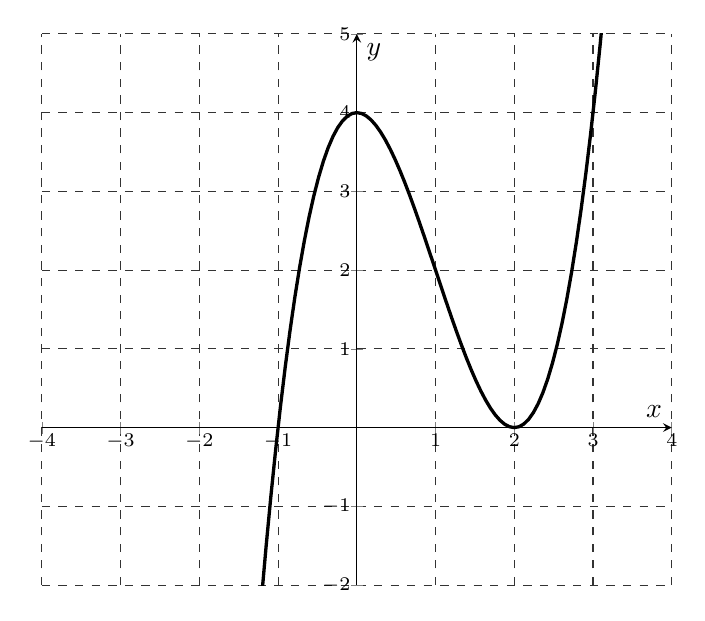
\begin{tikzpicture}
\begin{axis}[
	x=1cm,
	y=1cm,
	grid=major,
    ymin=-2,
    ymax=5,
    xmin=-4,
    xmax=4, 
    xlabel=$x$,
    ylabel=$y$,
    axis on top=true,
    axis x line=middle,
    axis y line=middle,
    axis on top = false,
    ]  
    
    \addplot [very thick, samples=100, domain=-2:4] {(x+1)*(x-2)^2};

\end{axis}
\end{tikzpicture} 
\end{center}

\begin{center}
\pgfplotsset{every tick label/.style={inner sep=0pt,font=\scriptsize}}
\pgfplotsset{grid style={dashed, black!80}}
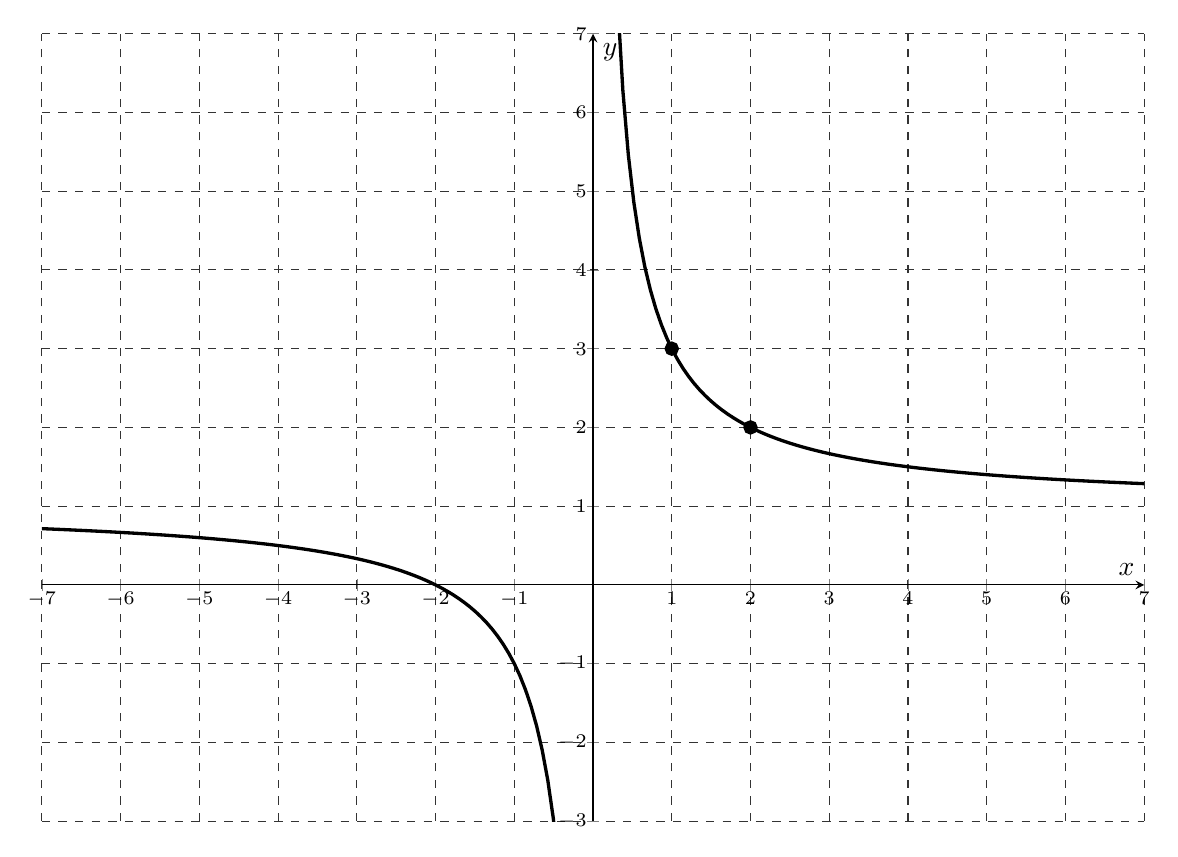
\begin{tikzpicture}
\begin{axis}[
	x=1cm,
	y=1cm,
	grid=major,
    ymin=-3,
    ymax=7,
    xmin=-7,
    xmax=7, 
    xlabel=$x$,
    ylabel=$y$,
    axis on top=true,
    axis x line=middle,
    axis y line=middle,
    axis on top = false,
    ]  
    
    \addplot [very thick, samples=100, domain=-7:-0.01] {2/x + 1};	%linker ast
     \addplot [very thick, samples=100, domain=0.1:7] {2/x + 1}; %rechter ast
     \addplot [very thick, only marks, samples=2, domain=1:2 ] {2/x + 1};   
\end{axis}	 %zwei markierte Punkte
\end{tikzpicture} 
\end{center}


\clearpage
\subsection*{Exponentialfunktion}

\begin{center}
\pgfplotsset{every tick label/.style={inner sep=0pt,font=\scriptsize}}
\pgfplotsset{grid style={dashed, black!80}}
\begin{tikzpicture}
\begin{axis}[
	%height=9cm,
	x=1cm,
	y=1cm,
	%grid=major,
    ymin=-3,
    ymax=7,
    xmin=-5,
    xmax=5, 
    ticks=none,
    legend pos= north west,
    xlabel=$x$,
    ylabel=$y$,
    axis on top=true,
    axis x line=middle,
    axis y line=middle,
    axis on top = false,
    ]  
    
    \addplot [very thick, dashed, samples=100, domain=-9:5] {2*1.7^x};
    \addlegendentry{$f(x) = 2 \cdot \num{1,7}^x$}
     \addplot [very thick, samples=100, domain=-9:5] {exp(x)};
    \addlegendentry{$g(x)= \ee^x$}
\end{axis}
\end{tikzpicture} 
\end{center}


\subsection*{Mit Hilfslinien}

 \begin{center}
\pgfplotsset{every tick label/.style={inner sep=0pt,font=\scriptsize}}
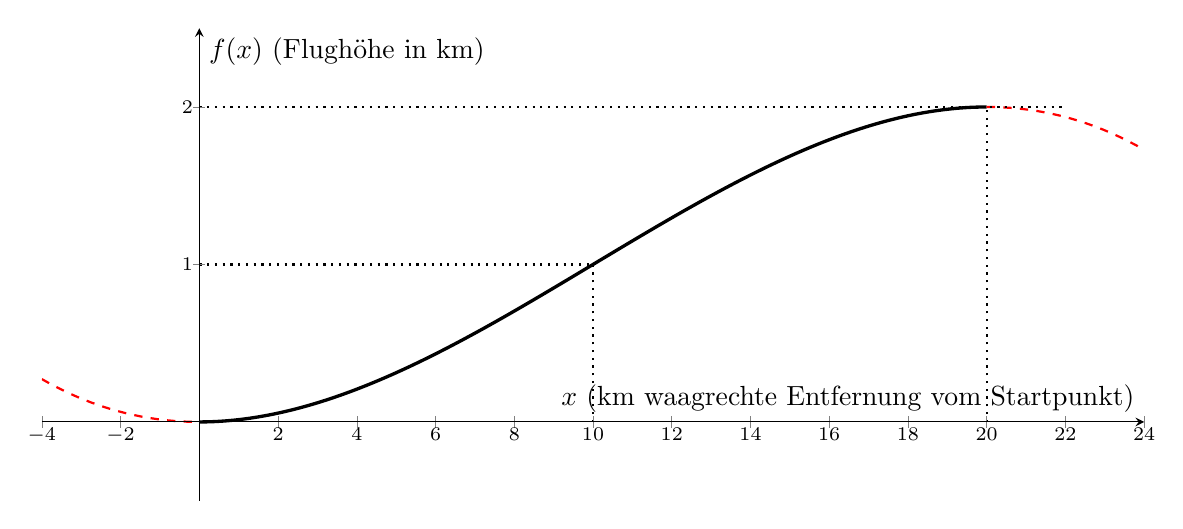
\begin{tikzpicture}
\begin{axis}[
	%height=9cm,
   x=0.5cm,
   y=2cm,
    ymin=-0.5,
    ymax=2.5,
    xmin=-4,
    xmax=24, 
    legend pos= south east,
    xlabel={$x$ (km waagrechte Entfernung vom Startpunkt)},
    ylabel=$f(x)$ (Flughöhe in km),
    axis on top=true,
    axis x line=middle,
    axis y line=middle
    ]  
    
    \addplot [very thick, samples=200,  domain=0:20] {-x^3/2000 + 3*x^2/200};
    \addplot [thick, dashed, color=red, samples=20,  domain=20:24] {-x^3/2000 + 3*x^2/200};
    \addplot [thick, dashed, color=red,  samples=20, domain=-4:0] {-x^3/2000 + 3*x^2/200};
   
	\draw [dotted, thick](axis cs: 0,2) -- (axis cs: 22,2);
	\draw [dotted, thick](axis cs: 20,0) -- (axis cs: 20,2);
	\draw [dotted, thick](axis cs: 10,0) -- (axis cs: 10,1);
	\draw [dotted, thick](axis cs: 0,1) -- (axis cs: 10,1);

\end{axis}
\end{tikzpicture} 
\end{center}

\clearpage
\subsection*{Zahlengerade mit tikz}

\begin{center}
\begin{tikzpicture}[line cap=round,line join=round,>=triangle 45,x=1cm,y=1cm]

\draw[<->,color=black] (-7.5,0) -- (7.5,0);

\foreach \x in {-7,-6, ..., 7}
\draw[shift={(\x,0)},color=black] (0pt,2pt) -- (0pt,-2pt) node[below] {\footnotesize $\x$};
\end{tikzpicture}
\end{center}


\subsection*{Komplexe Zahlenebene mit tikz}


\begin{center}
\begin{tikzpicture}[line cap=round,line join=round,>=triangle 45,x=0.75cm,y=0.75cm]

\fill [color = hellgrau!120] (-2,-2) rectangle(1, 2);
\draw [line width = 2pt, color = red](-2,-2) -- (-2,2);
\draw[->,color=black] (-5.,0.0) -- (6,0.0);

\foreach \x in {-5, -4, -3, -2, -1 , 1, 2, 3, 4,  5}
\draw[shift={(\x,0)},color=black] (0pt,2pt) -- (0pt,-2pt) node[below] {\footnotesize $\x$};

\draw[->,color=black] (0.0,-3) -- (0.0,5);
\foreach \y in {-2, -1, 1, 2, 3, 4}
\draw[shift={(0,\y)},color=black] (2pt,0pt) -- (-2pt,0pt) node[left] {\footnotesize $\y i$};
\end{tikzpicture}
\end{center}




\begin{center}
\begin{tikzpicture}[line cap=round,line join=round,>=triangle 45,x=0.75cm,y=0.75cm]

\filldraw[fill=hellgrau!120, draw=black, line width=0.1] (2,-3) circle (3);
\fill [color = white] (2,-3) circle (1);
\fill [color = black] (2,-3) circle (0.125);

\fill[fill=red,fill opacity=.6] (5,5.5) -- (-5,-4.5) -- (-5, -6.5) -- (5,3.5);
\draw[draw=black] (5,5.5) -- (-5,-4.5);

\fill[fill=yellow,fill opacity=.6] (-5,1) rectangle (5,2);
\draw[draw=black] (-5,1) -- (5,1);
\draw[draw=black] (-5,2) -- (5,2);

\draw (2,1.5) node {$K$};

%\draw [line width = 2pt, color = red](-2,-2) -- (-2,2);
\draw[->,color=black] (-5.,0.0) -- (5,0.0);

\foreach \x in {-5, -4, -3, -2, -1 , 1, 2, 3, 4,  5}
\draw[shift={(\x,0)},color=black] (0pt,2pt) -- (0pt,-2pt) node[below] {\footnotesize $\x$};

\draw[->,color=black] (0.0,-5) -- (0.0,5);
\foreach \y in {-6, -5, -4, -3, -2, -1, 1, 2, 3, 4}
\draw[shift={(0,\y)},color=black] (2pt,0pt) -- (-2pt,0pt) node[left] {\footnotesize $\y i$};

\end{tikzpicture}
\end{center}


